 !TeX root = ../main.tex
% Add the above to each chapter to make compiling the PDF easier in some editors.

\chapter{Einleitung}\label{chapter:introduction}
\todo{Alle Bildpositionen überprüfen!!!!}

	%Calculating the integral of a function $f(x)$ is a typical problem in numerics. In many cases, the function $f(x)$ is not known but only the function values at certain, potentially arbitrary, points. In this scenario, a common approach is to approximate the integral using the finite set of sampling points. This is a non-trivial problem.
	
	%The term \term{term} is marked like this for better understanding.
	
	%\todo{This marks a todo}{}
	Die Begriffe virtuelle Realität und erweiterte Realität kennen heutzutage viele Menschen. Allerdings wissen einige davon nicht wirklich was sich genau dahinter verbirgt. Dabei handelt es sich hierbei um zwei Forschungsbereiche, in welchen viele Firmen ein großes Potential sehen.\todo{Verweis} Noch sind sie zwar unwichtig für die meisten Privatnutzer, da die Anschaffung der bekanntesten notwendigen Geräte relativ kostspielig ist, aber In Zukunft werden diese Bereiche voraussichtlich auch dort noch weiter an Wichtigkeit gewinnen.
	Dies lässt sich bereits an den starken Entwicklungen auf dem Markt der sogenannten VR- und AR-Brillen in den letzten Jahren erkennen.
	Zwar gab es laut dem Marktforschungsunternehmen IDC einen Rückgang der Verkaufszahlen im Jahr 2018\todo{Verkaufszahlen rückgang zitieren}, die Prognosen für die kommenden Jahre sehen allerdings vielversprechend für diese Technologien aus, wie \refFigure{fig:forecast_diagram} zeigt.
	
	\begin{figure}[htbp]
		\centering
		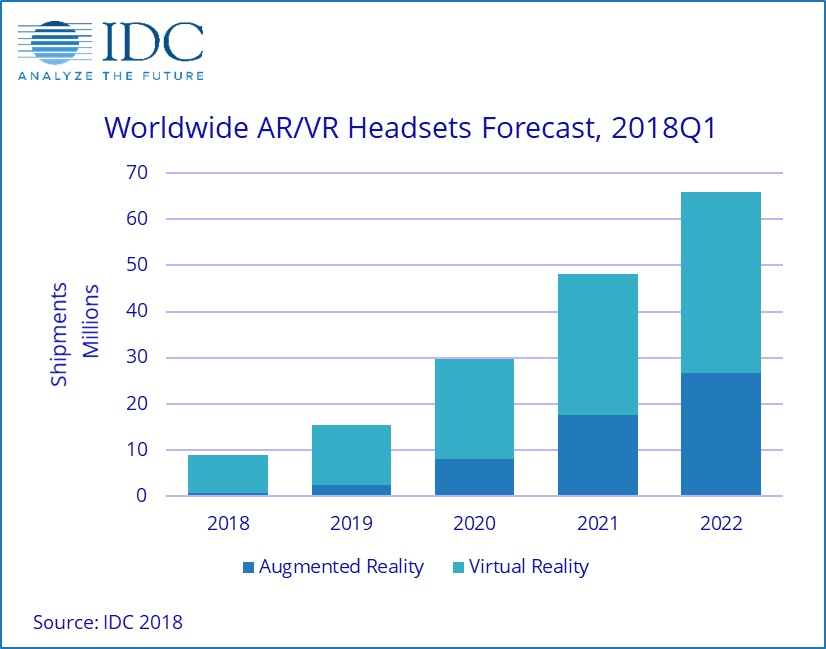
\includegraphics[width=0.6\textwidth]{figures/IDC-2018.jpg}
		\caption{Vorhersage der Verkaufszahlen nach IDC 2018 \takenFrom{asc_notes}.}
		\label{fig:forecast_diagram}
	\end{figure}
	
	Diese speziellen Brillen dienen als Medium, um Benutzern einen Einblick in eine teilweise oder gänzlich veränderte Welt zu geben.
	\todo{Mehr}
	Neben bereits bekannteren Exemplaren wie der HTC Vive von den Firmen HTC und Valve, der Oculus Rift von Oculus VR oder der Hololens von Microsoft, gibt es nun auch billigere Umsetzungen wie die Daydream View von Google, welche das eigene Smartphone als Display verwendet.\todo{Verweis} 
	Durch diese billigeren Varianten ist es auch mehr privaten Nutzern möglich ein eigenes VR-Gerät zu erwerben und auch zuhause einen Blick in virtuelle Welten zu werfen.
	- Angebot für jedermann (durch verschiedene Preiskategorien)
	- es wird davon ausgegangen, dass Handy-VR durch seine geringe Leistungsfähigkeit in Zukunft wieder zurückgehen wird
	Zudem werden weiterhin verbesserte Versionen älterer Geräte veröffentlicht. Ein Beispiel dafür ist die HTC Vive Pro, welche sowohl in der virtuellen als auch, im Gegensatz zu ihrem Vorgängermodell, in der erweiterten Realität angewendet werden kann.\todo{Referenz}

	Und auch bei den Programmen für diese Brillen hat sich viel getan...
	- Simulationen (Evtl Arbeit mit Drumset?)
	- verschiedene VR Spiele und Anwendungen Screenshots!
	- auch crossplay, aber bisher fast ohne UI
	\todo{Fortsetzen!}
	
	\section{Was ist VR/AR?}
	%- Augmented Reality = Erweiterte Realität
	%- Virtual Reality = Virtuelle oder künstliche Realität
	Bei der Definition von virtueller Realität (VR) und erweiterter Realität (AR, engl. Augmented Reality) und deren Abgrenzung zueinander gibt es relativ große Meinungsunterschiede. Der Designer \term{Tidjane Tall} zum Beispiel beschreibt diese beiden Begriffe in seinem Artikel \todo{Zitieren?} \term{Augmented Reality vs. Virtual Reality vs. Mixed Reality – An Introductory Guide} als zwei verschiedene Technologien, welche in Mixed Reality vereint werden. VR ist dabei eine Art Simulation, in der es dem Nutzer ermöglicht wird eine andere Umgebung zu sehen, als die, in der er sich tatsächlich befindet \todo{cite}. Die erweiterte Realität hingegen definiert er durch die Projizierung computergenerierter Objekte in die reale Umgebung in Form einer Maske, welche die Realität überlagert \todo{cite}. Dieses Prinzip wird beispielsweise in AR-Anwendungen für Smartphones verwendet \todo{Referenz}.
	
	Als Alternative dazu definiert \term{R. Azuma} die erweiterte Realität mit folgenden Eigenschaften... \todo{Aus Masterarbeit zweite AR quelle}
	-vermischung von real und virtuell
	-Echtzeitinteraktion
	-in der 3D Welt platziert
	
	%(Die virtuelle Realität (VR) und die erweiterte Realität (AR, engl. augmented reality) \todo{Checken wie das gemacht wird} bilden \todo{VR ist nicht Teilbereich sondern Grenze}) zwei Teilbereiche der Vermischung von virtueller Welt und Realität, der sogenannten Mixed Reality (MR). Bei der genauen Definition von virtueller und erweiterter Realität, sowie deren Abgrenzung voneinander, unterscheiden sich die Meinungen der ... \todo{Formulierung finden}
	
	
	Eine der verbreitetsten Definitionen stammt allerdings von \term{Milgram et al.} aus deren Arbeit \term{Titel} \todo{Zitat Milgram} ... Dabei wird der Bereich der Mixed-Reality als der Übergang zwischen der realen Welt und der virtuellen Welt definiert. Die beiden Enden zählen allerdings jeweils nicht zu diesem sogenannten Reality-Virtuality Continuum\cite{milgram}. Dieses Modell veranschaulicht \refFigure{fig:mixed_reality}. Dabei sieht man allerdings ebenfalls, dass die erweiterte Realität innerhalb des Kontinuums nicht weiter eingegrenzt wurde.
	
	\begin{figure}[htbp]
		\centering
		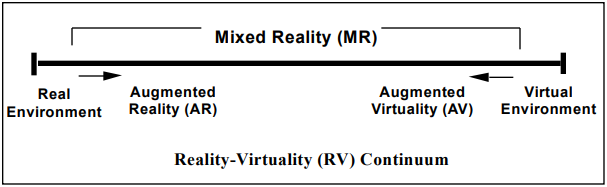
\includegraphics[width=0.75\textwidth]{figures/mixed_reality.png}
		\caption{Example picture that was taken from an external source \takenFrom{milgram}.}
		\label{fig:mixed_reality}
	\end{figure}
	\todo{Untertitel bearbeiten}
	
	%- Head Mounted Display
	%- Mischung von Realität und virtuellen Elementen
	%- AR lebt von der realen Welt und somit von freiem Bewegen
	%-> nicht an Pc gebunden
	--> weniger Leistung
	--> kein Handtracking
	
	Zur Umsetzung von VR und AR gab es in der Vergangenheit bereits mehrere Ideen, welche auf unterschiedliche Szenarien zugeschnitten sind.
	- Beispiel HUD (was ebenso noch Verwendung findet)
	Die Variante mit einem HMD (Head Mounted Device)\todo{Checken} hat sich bisher allerdings in vielen Bereichen durchgesetzt, da sie ein hohes Maß an Immersion bietet und dabei nicht zwingend viel Platz verbraucht \todo{Verweis}. Außerdem kann man sich mit einem HMD relativ frei im Raum bewegen, auch wenn einige Modelle aus Gründen der Leistungsfähigkeit eine Verbindung zu einem Rechner benötigen und somit nur in der Nähe von diesem verwendet werden können. Dies ist ebenso bei der Verwendung von System zur Positionserfassung des HMDs oder der verwendeten Controller der Fall, da diese Systeme normalerweise statisch in der Welt platziert sind. Da die erweiterte Realität allerdings von der realen Welt lebt, gibt es Bemühungen die Notwendigkeit eines stationären Computers zu entfernen, ohne dabei die Performanz zu mindern. - Hololens
	Dadurch 

	\section{Was ist eine Benutzeroberfläche?}
		%- Schnittstelle zwischen Nutzer und Programm
		Im Bereich der Mensch-Maschine-Interaktion, kurz HCI (Human-Computer-Interaction) wird im Groben zwischen drei Bereichen unterschieden: Mensch, Maschine und deren Schnittstelle.\linebreak
		Die Benutzeroberfläche \todo{In Klammern: englisch user interface, UI} stellt eben jenen Übergang zwischen Maschine und Mensch dar und ermöglicht die Interaktion beider Seiten miteinander.\todo{Verweise!}
		%- nur die graphische Seite GUI betrachtet
		Sie lässt sich weiter in physische Steuerelemente und graphische Bestandteile (das GUI, engl. graphical user interface)\todo{Übersetzungen handhaben} aufteilen. Zu dem ersten Bereich zählen alle Arten von Knöpfen, Hebeln, Reglern und Sensoren, welche Eingaben durch den Nutzer ermöglichen, ebenso wie visuelle, haptische oder akustische Ausgabegeräte, welche dem Nutzer eine Rückmeldung zu dessen Aktionen geben und den Status des ausgeführten Programms an den Benutzer weiterleiten.\todo{Fortsetzen}
		- graphischer Bereich hat frühere Kommandozeile abgelöst und Verwendung vereinfacht
		- in Form einer Maske, welche über den Rest gelegt wird
		Der 
		In dieser Arbeit wird allerdings nur der graphische Anteil betrachtet.
		
		%-Stellt Information zur Verfügung und ermöglicht die Erfassung und Manipulation der virtuellen Umgebung
		Er stellt dem Nutzer über Texte, Bilder und Farben Informationen zur Verfügung und kann deren Manipulation ermöglichen. Damit soll Benutzern die Erfassung und Veränderung der virtuellen Umgebung erleichtert werden.
		- Häufig als Menüs
		
		Eine spezielle Form der graphischen Benutzeroberfläche ist die dreidimensionale Benutzeroberfläche
	
		\subsection{Element}
			%- Beispiele: Textfeld, Bild, Schaltfläche...
			Die graphische Benutzeroberfläche setzt sich aus einzelnen Elementen zusammen. Diese können beispielsweise Texte, Bilder oder Schaltflächen sein, welche normalerweise innerhalb einer Menüstruktur untereinander oder nebeneinander angeordnet sind.
			\todo{Mehr! Anker erwähnen}
	
		\subsection{Anker}
			%- Position an welcher Elemente der Benutzeroberfläche platziert werden
			Ein Anker bezeichnet eine Position, zu welcher die Elemente der Benutzeroberfläche relativ platziert werden.
			\todo{Noch mehr dazu schreiben? Verweise suchen!}
			- In Desktop-Programmen werden dafür meist die Bildschirmkanten beziehungsweise Ecken verwendet
			%-Beispiel aus Unity
			\begin{figure}[htbp]
				\centering
				\includegraphics[width=0.4\textwidth]{figures/Ui_Anchor_Unity.png}
				\caption{Beispiel aus Unity that was taken from an external source \takenFrom{asc_notes}.}
				\label{fig:unity}
			\end{figure}
			\todo{Untertitel bearbeiten}
			
			An dem Beispiel aus der Spiel-Engine Unity (siehe \refFigure{fig:unity}), sieht man die möglichen Ankerpositionen innerhalb des Anwendungsfensters.  \todo{Weiter}
			
			In dieser Arbeit wurden als Ankerpunkte die beiden Handpositionen des Benutzers und die Kopfposition verwendet, da diese Stellen im Fall von...
	
	\section{Was bedeutet umgebungsabhängig?}
		%- UI befindet sich im 3D Raum und kann von Objekten verdeckt werden. Sie ist an eine 3D Position gebunden und kann sich unabhängig vom Benutzer verschieben und rotieren, sie muss also nicht statisch zur Kamera sein
		Als umgebungsabhängig werden in dieser Arbeit Benutzeroberflächen bezeichnet, welche sich, im Gegensatz zum herkömmlichen zweidimensionalen Äquivalent, im dreidimensionalen Raum befinden und somit auch von Objekten aus der virtuellen oder realen Umgebung verdeckt werden können. Sie sind somit nicht wie eine Maske, die zwischen Kamera und der Umgebung angezeigt wird, sondern wie Bestandteile der, den Nutzer umgebenden, Welt. Zudem müssen sie sich nicht statisch zu, beziehungsweise abhängig von, der Kamera bewegen, sondern können auch an einen anderen Gegenstand aus der Umgebung gebunden werden, mit dem sie sich mitbewegen und gegebenenfalls mitrotieren.
		- In 3D Programmen wird solche UI meist an Objekten positioniert und ist zu diesen statisch \todo{Verweis}, es handelt sich dabei meist um (diegetic?)
	